%%%%%%%%%%%%%%%%%%%%%%%%%%%%%%%%%%%%%%%%%
% Beamer Presentation
% LaTeX Template
% Version 1.0 (10/11/12)
%
% This template has been downloaded from:
% http://www.LaTeXTemplates.com
%
% License:
% CC BY-NC-SA 3.0 (http://creativecommons.org/licenses/by-nc-sa/3.0/)
%
%%%%%%%%%%%%%%%%%%%%%%%%%%%%%%%%%%%%%%%%%

%----------------------------------------------------------------------------------------
%	PACKAGES AND THEMES
%----------------------------------------------------------------------------------------

\documentclass{beamer}

\mode<presentation> {

% The Beamer class comes with a number of default slide themes
% which change the colors and layouts of slides. Below this is a list
% of all the themes, uncomment each in turn to see what they look like.

%\usetheme{default}
%\usetheme{AnnArbor}
%\usetheme{Antibes}
%\usetheme{Bergen}
%\usetheme{Berkeley}
%\usetheme{Berlin}
%\usetheme{Boadilla}
%\usetheme{CambridgeUS}
%\usetheme{Copenhagen}
%\usetheme{Darmstadt}
%\usetheme{Dresden}
%\usetheme{Frankfurt}
%\usetheme{Goettingen}
%\usetheme{Hannover}
%\usetheme{Ilmenau}
%\usetheme{JuanLesPins}
%\usetheme{Luebeck}
\usetheme{Madrid}
%\usetheme{Malmoe}
%\usetheme{Marburg}
%\usetheme{Montpellier}
%\usetheme{PaloAlto}
%\usetheme{Pittsburgh}
%\usetheme{Rochester}
%\usetheme{Singapore}
%\usetheme{Szeged}
%\usetheme{Warsaw}

% As well as themes, the Beamer class has a number of color themes
% for any slide theme. Uncomment each of these in turn to see how it
% changes the colors of your current slide theme.

%\usecolortheme{albatross}
%\usecolortheme{beaver}
%\usecolortheme{beetle}
%\usecolortheme{crane}
%\usecolortheme{dolphin}
%\usecolortheme{dove}
%\usecolortheme{fly}
%\usecolortheme{lily}
%\usecolortheme{orchid}
%\usecolortheme{rose}
%\usecolortheme{seagull}
%\usecolortheme{seahorse}
%\usecolortheme{whale}
%\usecolortheme{wolverine}

%\setbeamertemplate{footline} % To remove the footer line in all slides uncomment this line
%\setbeamertemplate{footline}[page number] % To replace the footer line in all slides with a simple slide count uncomment this line

%\setbeamertemplate{navigation symbols}{} % To remove the navigation symbols from the bottom of all slides uncomment this line
}

\usepackage{graphicx} % Allows including images
\usepackage{booktabs} % Allows the use of \toprule, \midrule and \bottomrule in tables
\usepackage{multirow}
\usepackage{adjustbox}
\usepackage{array}
\usepackage{tikz}
\usepackage{soul}
\usepackage{pdfpages}
\usetikzlibrary{shapes.geometric, arrows, positioning, fit}
\usepackage[latin1]{inputenc}
\newcommand{\xmark}{\textcolor{red}{\text{\sffamily X}}}
\newcommand{\cmark}{\textcolor{green}{\checkmark}}
\newcommand{\tr}{\text{tr}}
\newcommand{\E}{\textbf{E}}
\newcommand{\diag}{\text{diag}}
\newcommand{\argmax}{\text{argmax}}
\newcommand{\argmin}{\text{argmin}}
\newcommand{\Cov}{\text{Cov}}
\newcommand{\Var}{\text{Var}}
\newcommand{\Vol}{\text{Vol}}
\newcommand{\bx}{\boldsymbol{x}}
\newcommand{\by}{\boldsymbol{y}}
\newcommand{\bX}{\boldsymbol{X}}
\newcommand{\bY}{\boldsymbol{Y}}
\sethlcolor{gray}
\makeatletter
\newcommand\SoulColor{%
  \let\set@color\beamerorig@set@color
  \let\reset@color\beamerorig@reset@color}
\makeatother
\definecolor{color1}{RGB}{128,13,13}
\definecolor{color2}{RGB}{70,128,13}
\definecolor{color3}{RGB}{13,128,128}
\definecolor{color4}{RGB}{70,13,128}

%tikz stufff


%----------------------------------------------------------------------------------------
%	TITLE PAGE
%----------------------------------------------------------------------------------------


\title[Inference through learning]{What does classification tell us about the brain? Statistical inference through machine learning}

\author{Charles Zheng} % Your name
\institute[Stanford] % Your institution as it will appear on the bottom of every slide, may be shorthand to save space
{Stanford University}
\date{\today} % Date, can be changed to a custom date

\begin{document}

\begin{frame}
\titlepage % Print the title page as the first slide
(Joint work with Yuval Benjamini.)
\end{frame}

\section{Introduction}

%\begin{frame}
%\frametitle{Dependence, distance, and information}
%\begin{columns}
%\begin{column}{0.5\textwidth}
%\begin{center}
%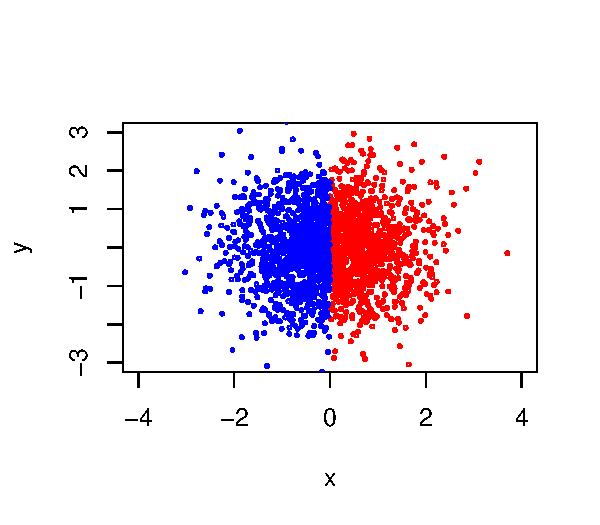
\includegraphics[scale = 0.4, clip = true, trim = 0.1in 0.1in 0.1in 0.2in]{../diagram/ddi_1a.pdf}
%\end{center}
%\begin{itemize}
%\item $X$ is independent of $Y$: 
%\[X \perp Y\]
%\item $X$ and $Y$ have no mutual information:
%\[
%I(X; Y) = 0
%\]
%\end{itemize}
%\end{column}
%\begin{column}{0.5\textwidth}
%\end{column}
%\end{columns}
%\end{frame}



%\begin{frame}
%\frametitle{Dependence, distance, and information}
%\begin{columns}
%\begin{column}{0.5\textwidth}
%\begin{center}
%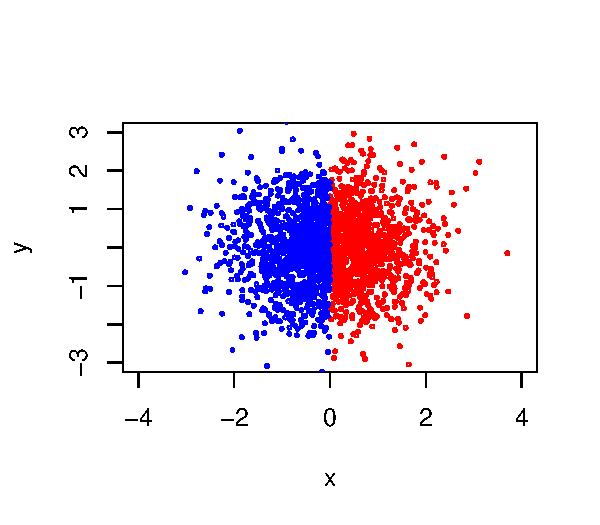
\includegraphics[scale = 0.4, clip = true, trim = 0.1in 0.1in 0.1in 0.2in]{../diagram/ddi_1a.pdf}
%\end{center}
%\begin{itemize}
%\item $X$ is independent of $Y$: 
%\[X \perp Y\]
%\item $X$ and $Y$ have no mutual information:
%\[
%I(X; Y) = 0
%\]
%\end{itemize}
%\end{column}
%\begin{column}{0.5\textwidth}
%\begin{center}
%Classifying $\text{Sign}(X)$ from $Y$

%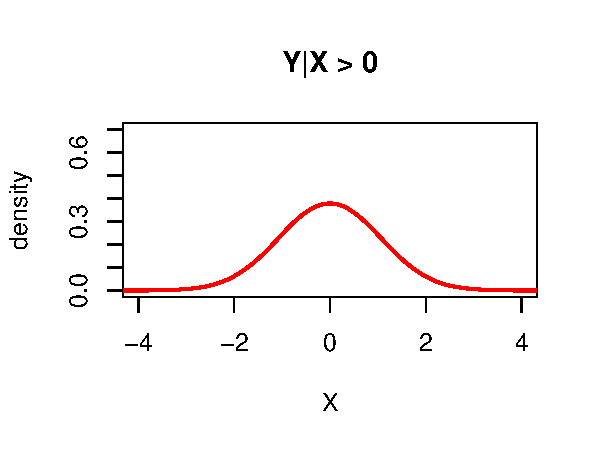
\includegraphics[scale = 0.4, clip = true, trim = 0.1in 0.9in 0.1in 0.2in]{../diagram/ddi_1b.pdf}

%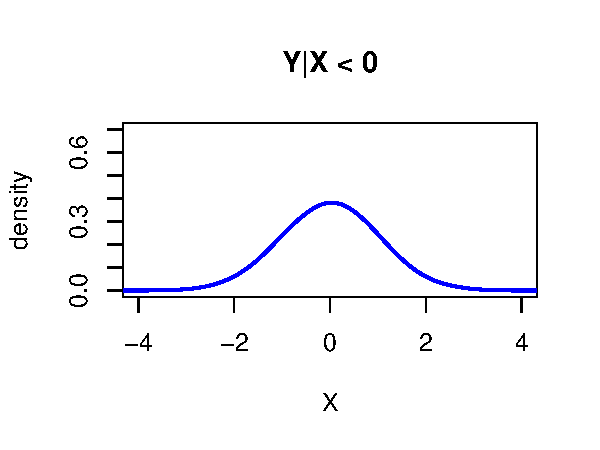
\includegraphics[scale = 0.4, clip = true, trim = 0.1in 0.1in 0.1in 0.2in]{../diagram/ddi_1c.pdf}
%\end{center}
%$KL(Y|X > 0, Y|X < 0) = 0.$

%Bayes accuracy = 0.5.
%\end{column}
%\end{columns}
%\end{frame}

\begin{frame}
\frametitle{Dependence, information}
\begin{columns}
\begin{column}{0.5\textwidth}
\begin{center}
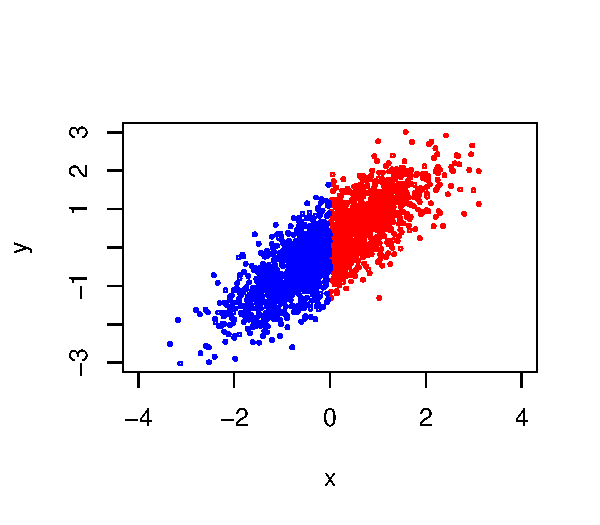
\includegraphics[scale = 0.4, clip = true, trim = 0.1in 0.1in 0.1in 0.2in]{../diagram/ddi_2a.pdf}
\end{center}
\begin{itemize}
\item $X$ is dependent of $Y$.
\item $X$ and $Y$ have mutual information:
\[
I(X; Y) = 0.51.
\]
\end{itemize}
\end{column}
\begin{column}{0.5\textwidth}
\end{column}
\end{columns}
\end{frame}

\begin{frame}
\frametitle{Dependence, information, and classification}
\begin{columns}
\begin{column}{0.5\textwidth}
\begin{center}
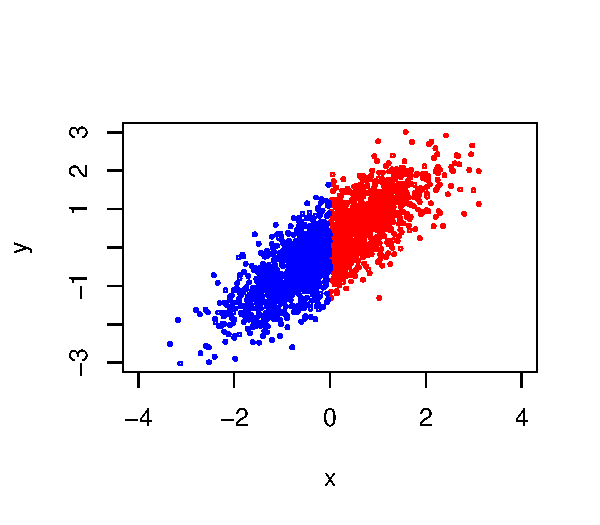
\includegraphics[scale = 0.4, clip = true, trim = 0.1in 0.1in 0.1in 0.2in]{../diagram/ddi_2a.pdf}
\end{center}
\begin{itemize}
\item $X$ is dependent of $Y$.
\item $X$ and $Y$ have mutual information:
\[
I(X; Y) = 0.51.
\]
\end{itemize}
\end{column}
\begin{column}{0.5\textwidth}
\begin{center}
Classifying $\text{Sign}(X)$ from $Y$

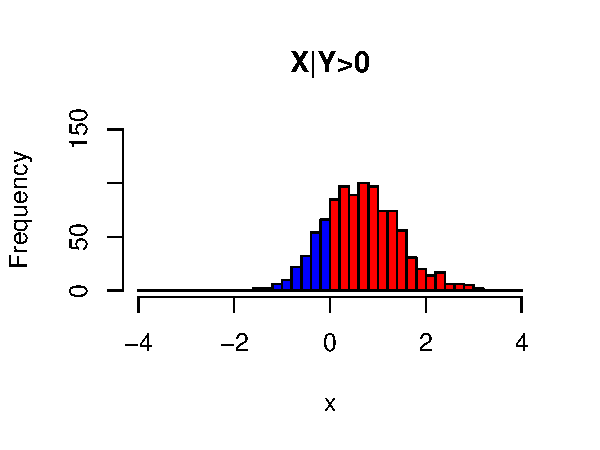
\includegraphics[scale = 0.4, clip = true, trim = 0.1in 0.9in 0.1in 0.2in]{../diagram/ddi_2b.pdf}

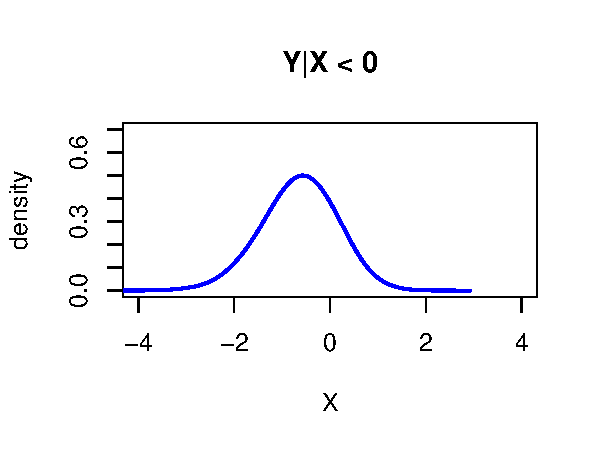
\includegraphics[scale = 0.4, clip = true, trim = 0.1in 0.1in 0.1in 0.2in]{../diagram/ddi_2c.pdf}
\end{center}

Bayes accuracy = 0.795.
\end{column}
\end{columns}
\end{frame}

\begin{frame}
\frametitle{Bayes accuracy}
\begin{itemize}
\item Discrete $Y \in \{1,...,k\}$, continuous or discrete $X$.
\item A classifier is a function $f$ mapping $x$ to a label in $\{1,..,k\}$
\item Generalization accuracy of the classifier:
\[
\text{GA}(f) = \Pr[Y = f(x)]
\]
\item Bayes accuracy:
\[
\text{BA} = \sup_f \Pr[Y = f(x)] = \Pr[Y = \text{argmax}_{i=1} p(X|Y=i)]
\]
\item Since random guessing is correct with probability $1/k$,
\[
\text{BA} \in [1/k, 1]
\]
(if $Y$ is uniformly distributed)
\end{itemize}
\end{frame}


\begin{frame}
\frametitle{Mutual information}
\begin{itemize}
\item Invented by Claude Shannon; central to \emph{information theory}.
\item Given $(X, Y)$ with joint density $p(x, y)$,
\[
I(X; Y) = \int p(x, y) \log\frac{p(x, y)}{p(x) p(y)} dx dy
\]
where $p(x)$ and $p(y)$ are marginal densities.
\end{itemize}
\end{frame}

\begin{frame}
\frametitle{Mutual information}
\begin{center}
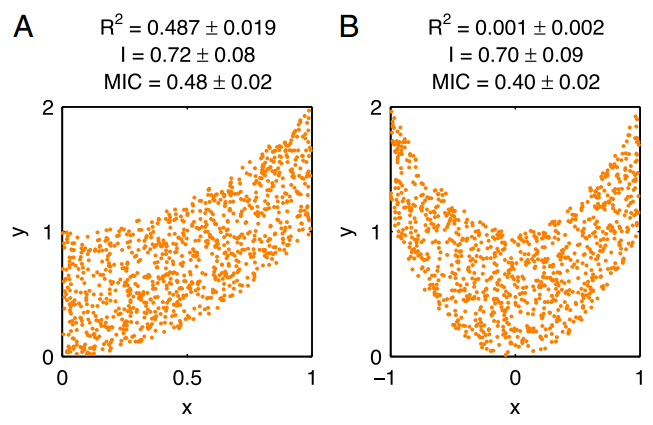
\includegraphics[scale = 0.2]{kinney.png}
\end{center}
\begin{itemize}
\item $I(X;Y) \in [0,\infty]$.  (0 if $X \perp Y$, $\infty$ if $X=Y$ and $X$ continuous.)
\item Symmetry: $I(X;Y) = I(Y; X)$.
\item Data-processing inequality
\[I(X; Y) \geq I(\phi(X); \psi(Y))\]
equality for $\phi$, $\psi$ bijections
\item Additivity.  If $(X_1,Y_1) \perp (X_2, Y_2)$, then
\[
I((X_1, X_2); (Y_1, Y2)) = I(X_1; Y_1) + I(X_2; Y_2).
\]
%\item Relation to KL divergence
%\[\mathbb{D}(p(x, y)||p(x)p(y)) = I(X; Y).\]
\end{itemize}
\tiny{Image credit Kinney et al. 2014.}
\end{frame}

\begin{frame}
\frametitle{Informativity of predictor sets}

Consider predicting binary $Y$ with:
\begin{itemize}
\item $X_1$ only
\item $X_1$ and $X_2$
\item $X_1, ..., X_k$
\end{itemize}

\begin{center}
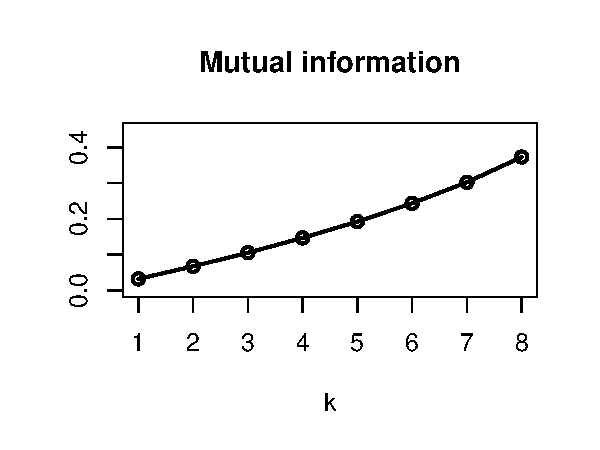
\includegraphics[scale = 0.6, clip = true, trim = 0.1in 0.1in 0.1in 0.2in]{../diagram/informativity1.pdf}
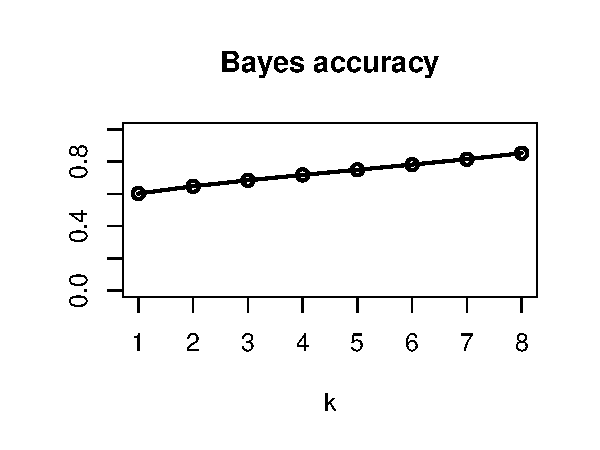
\includegraphics[scale = 0.6, clip = true, trim = 0.1in 0.1in 0.1in 0.2in]{../diagram/informativity2.pdf}
\end{center}

\end{frame}

\begin{frame}
\frametitle{Mutual information vs Bayes accuracy}
\begin{itemize}
\item Both are measures of ``informativity''.
\item Due to its properties, mutual information is easier to interpret.
\item Both are intractable to estimate in high dimensions.
\item However, Bayes accuracy has a tractable \emph{lower bound}: the generalization error of \emph{any} classifier.
\end{itemize}
\end{frame}

\begin{frame}
\frametitle{Studying the neural code}
\begin{center}
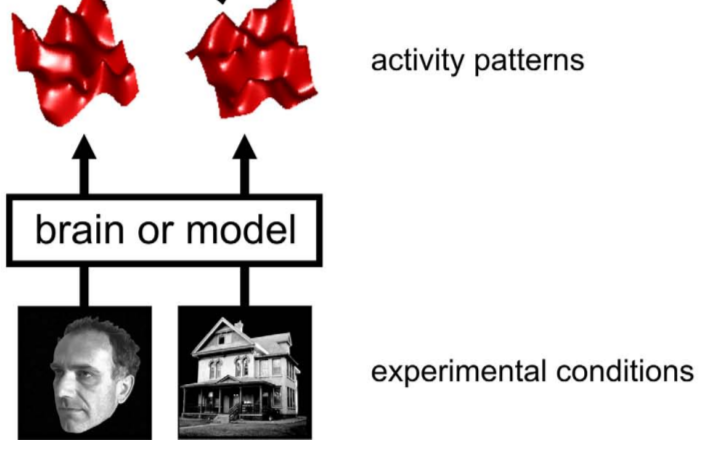
\includegraphics[scale = 0.3]{k08_step1.png}
\end{center}
Present the subject with visual stimuli, pictures of faces and houses.
Record the subject's brain activity in the fMRI scanner.
\end{frame}

%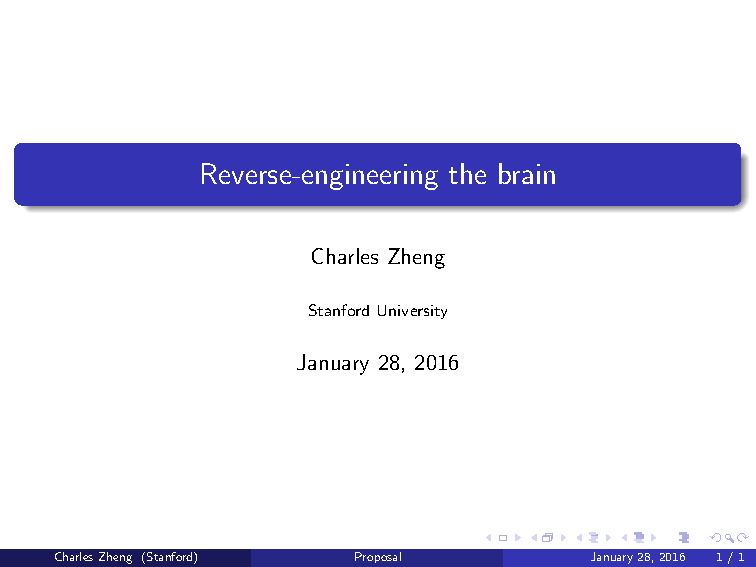
\includepdf[pages=1]{Zheng_proposal.pdf}
{
\setbeamercolor{background canvas}{bg=}
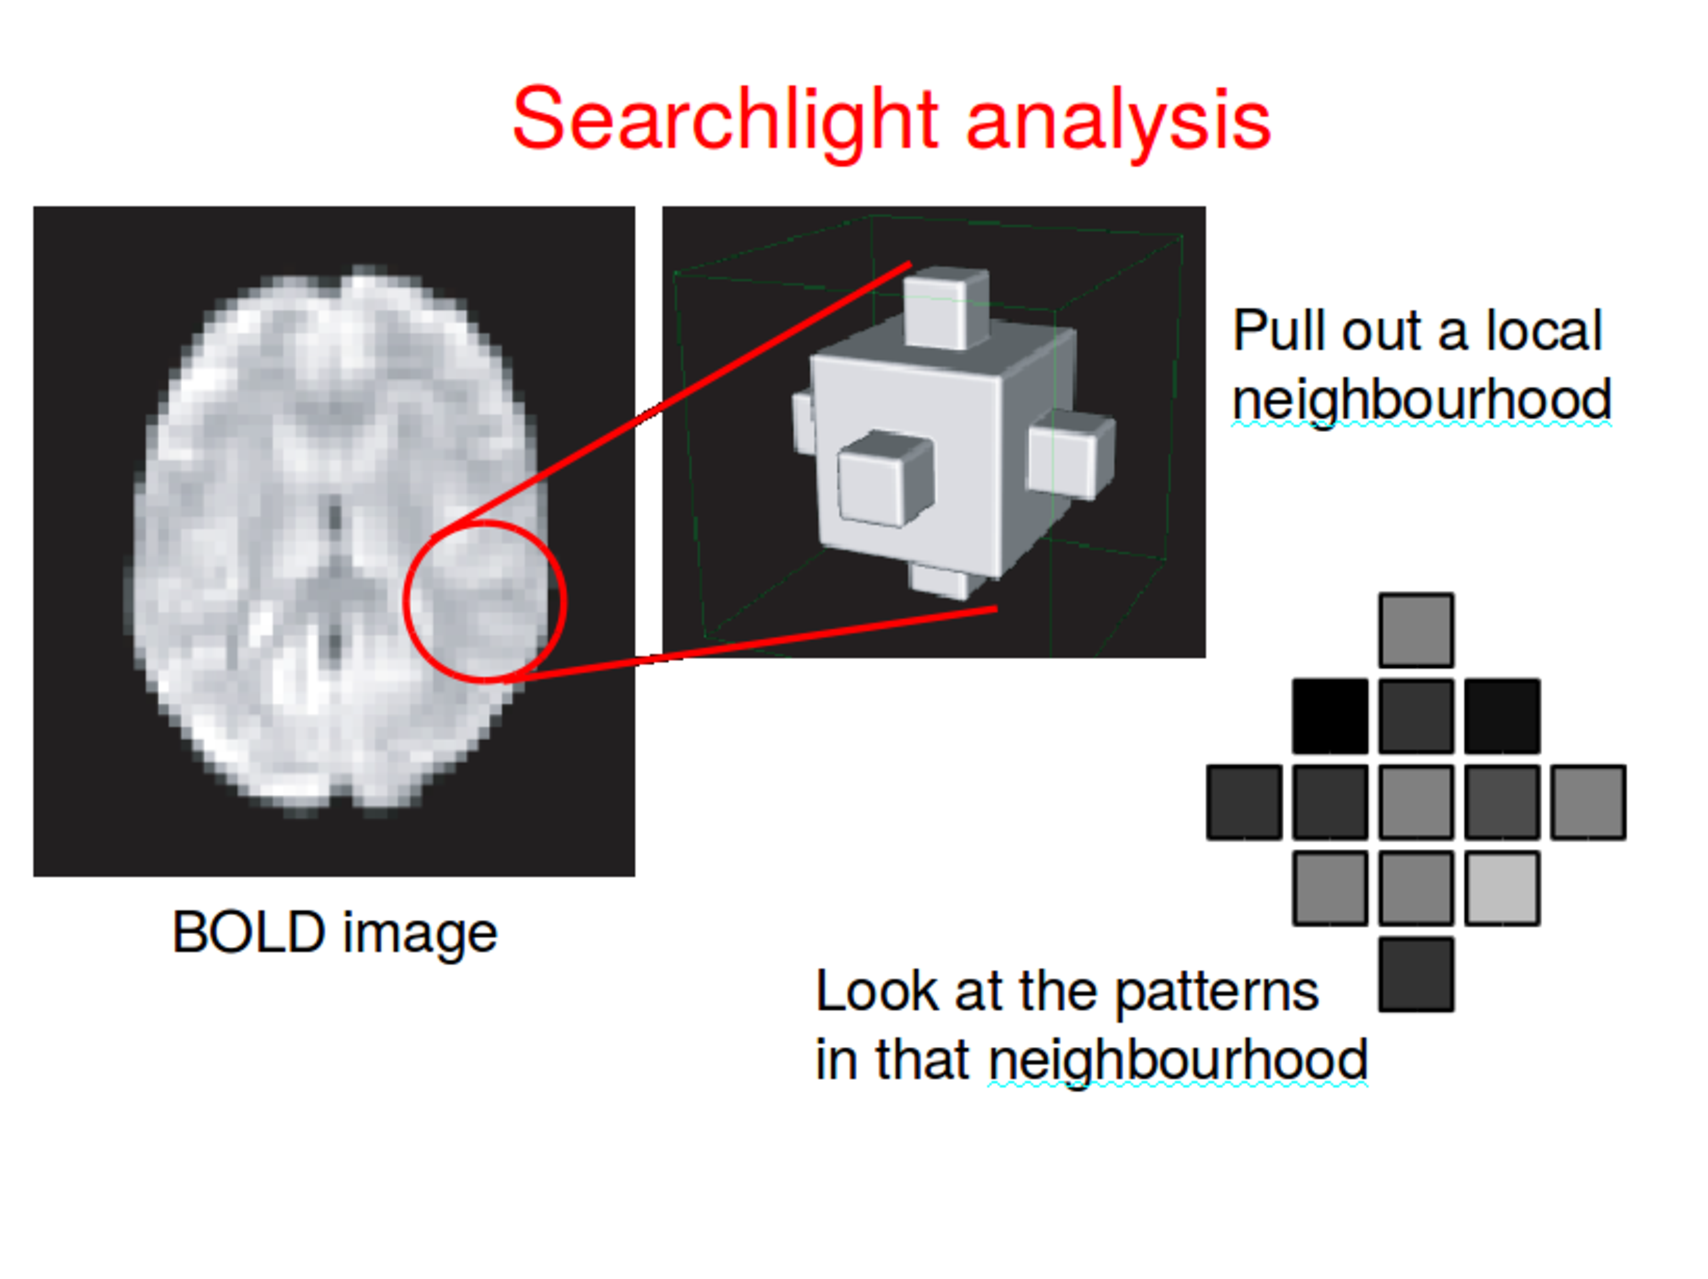
\includepdf[pages=1]{searchlight_slide.pdf}
% from Razaida
}

\begin{frame}
\frametitle{Searchlight analysis}
\begin{center}
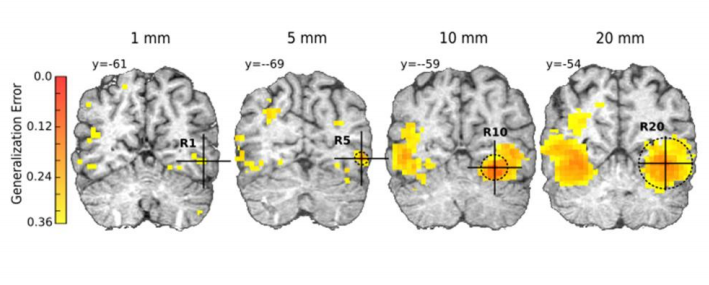
\includegraphics[scale = 0.5]{searchlight_windowsize.png}
\end{center}
Produces a map of ``informative'' regions of the brain (as measured by generalization accuracy).
\end{frame}

{
\setbeamercolor{background canvas}{bg=}
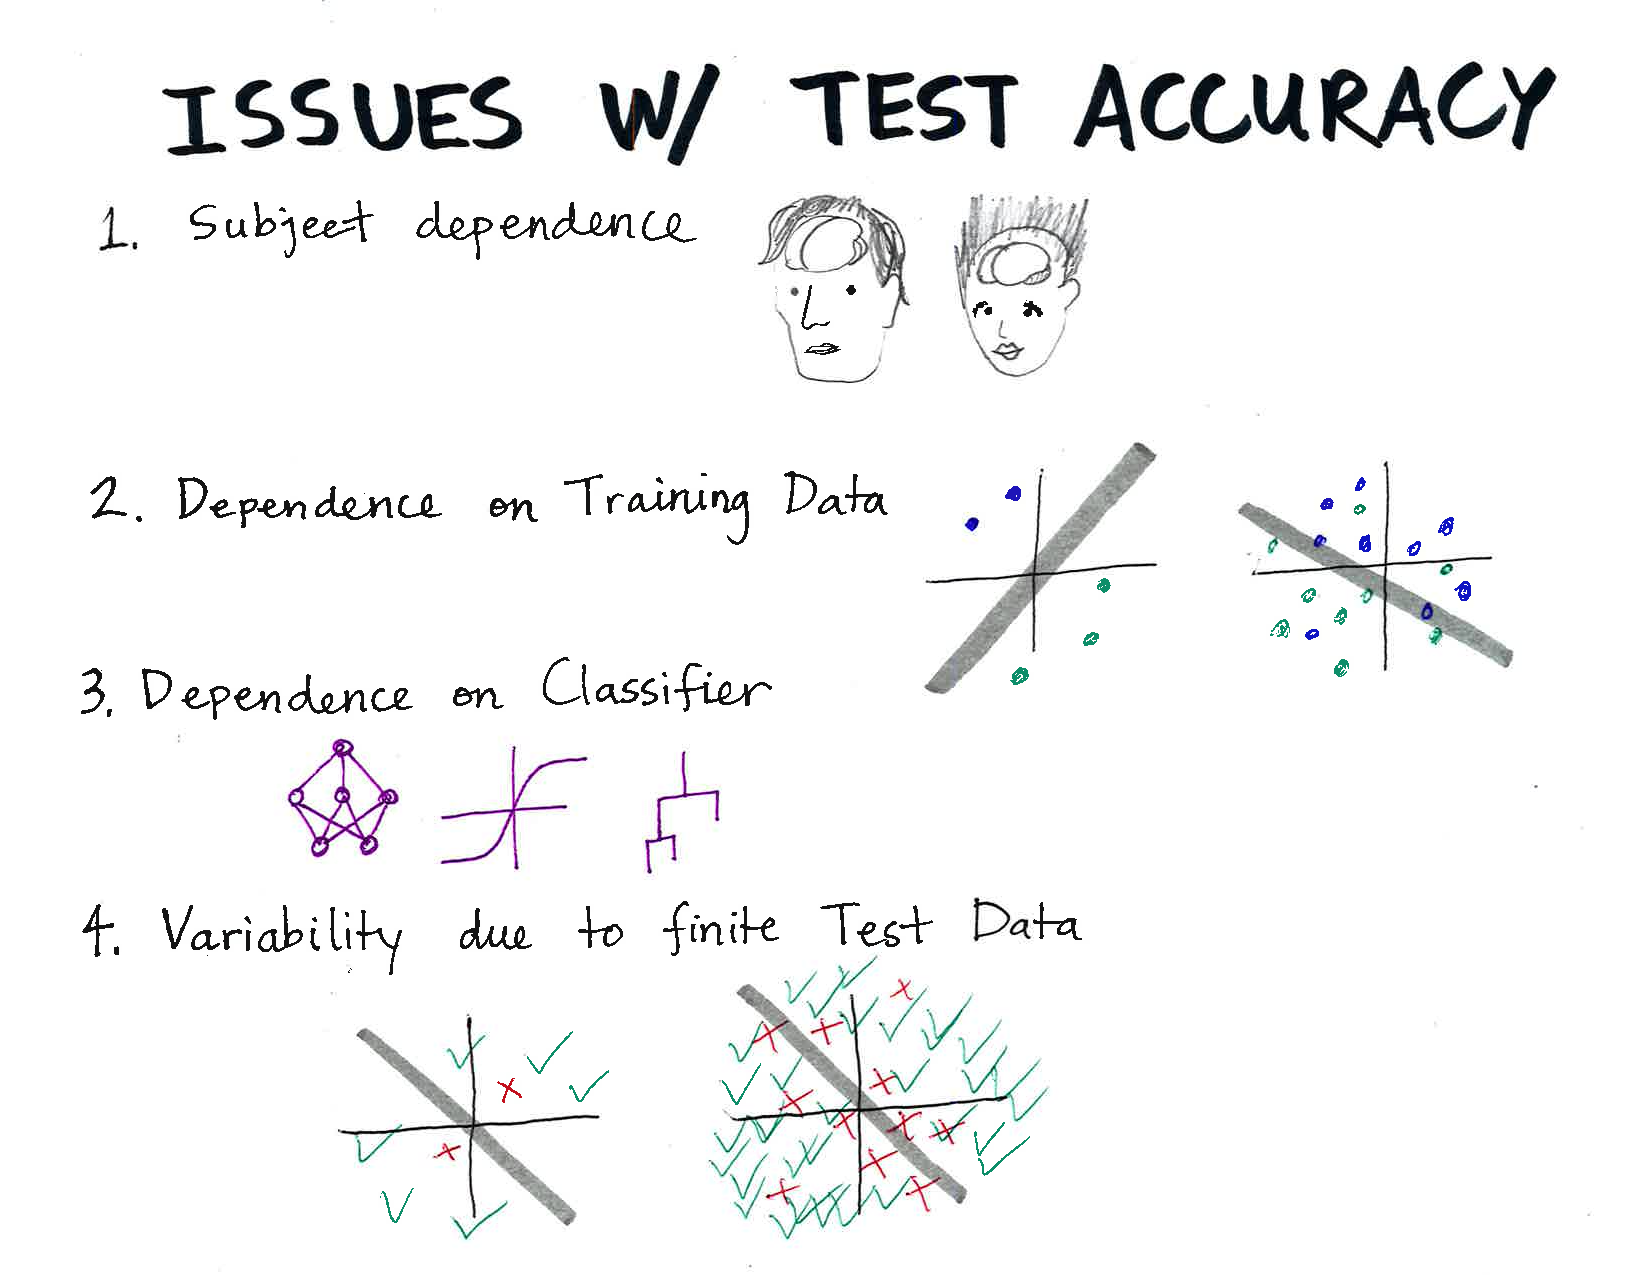
\includepdf[pages=1-2]{drawings_einstein.pdf}
% from Razaida
}

\begin{frame}
\frametitle{Fixed classification task}
\begin{columns}
\begin{column}{0.6\textwidth}
\begin{tabular}{cc}
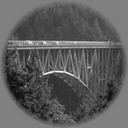
\includegraphics[scale = 0.5]{img1.png} &
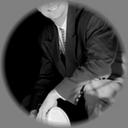
\includegraphics[scale = 0.5]{img2.png} \\
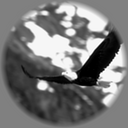
\includegraphics[scale = 0.5]{img3.png} &
\end{tabular}
\end{column}
\begin{column}{0.4\textwidth}
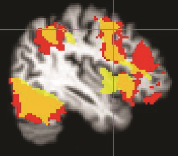
\includegraphics[scale = 0.5]{smbrain1.png}
\end{column}
\end{columns}
\begin{itemize}
\item Different stimuli sets lead to different \emph{Bayes accuracy}.
\end{itemize}
\end{frame}

\begin{frame}
\frametitle{Fixed classification task}
\begin{columns}
\begin{column}{0.6\textwidth}
\begin{tabular}{cc}
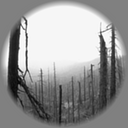
\includegraphics[scale = 0.5]{img5.png} &
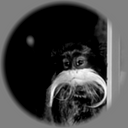
\includegraphics[scale = 0.5]{img6.png} \\
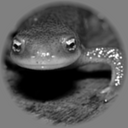
\includegraphics[scale = 0.5]{img7.png} &
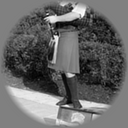
\includegraphics[scale = 0.5]{img8.png}
\end{tabular}
\end{column}
\begin{column}{0.4\textwidth}
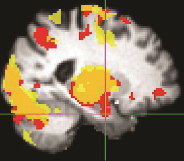
\includegraphics[scale = 0.5]{smbrain2.png}
\end{column}
\end{columns}
\begin{itemize}
\item Different stimuli sets lead to different \emph{Bayes accuracy}.
\item Results are incomparable, even in the large-sample limit.
\end{itemize}
\end{frame}

\begin{frame}
\frametitle{Generalizing beyond the design}

\begin{columns}
\begin{column}{0.6\textwidth}
\begin{center}
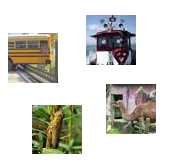
\includegraphics[scale = 1]{imagenet_sub.png}
\end{center}
\end{column}
\begin{column}{0.4\textwidth}
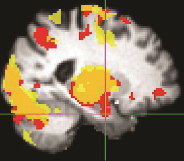
\includegraphics[scale = 0.5]{smbrain2.png}
\end{column}
\end{columns}

Scientists are not innately interested in the Bayes accuracy of a \emph{particular} stimuli set, which is often chosen arbitrarily...

\end{frame}

\begin{frame}
\frametitle{Generalizing beyond the design}

\begin{columns}
\begin{column}{0.6\textwidth}
\begin{center}
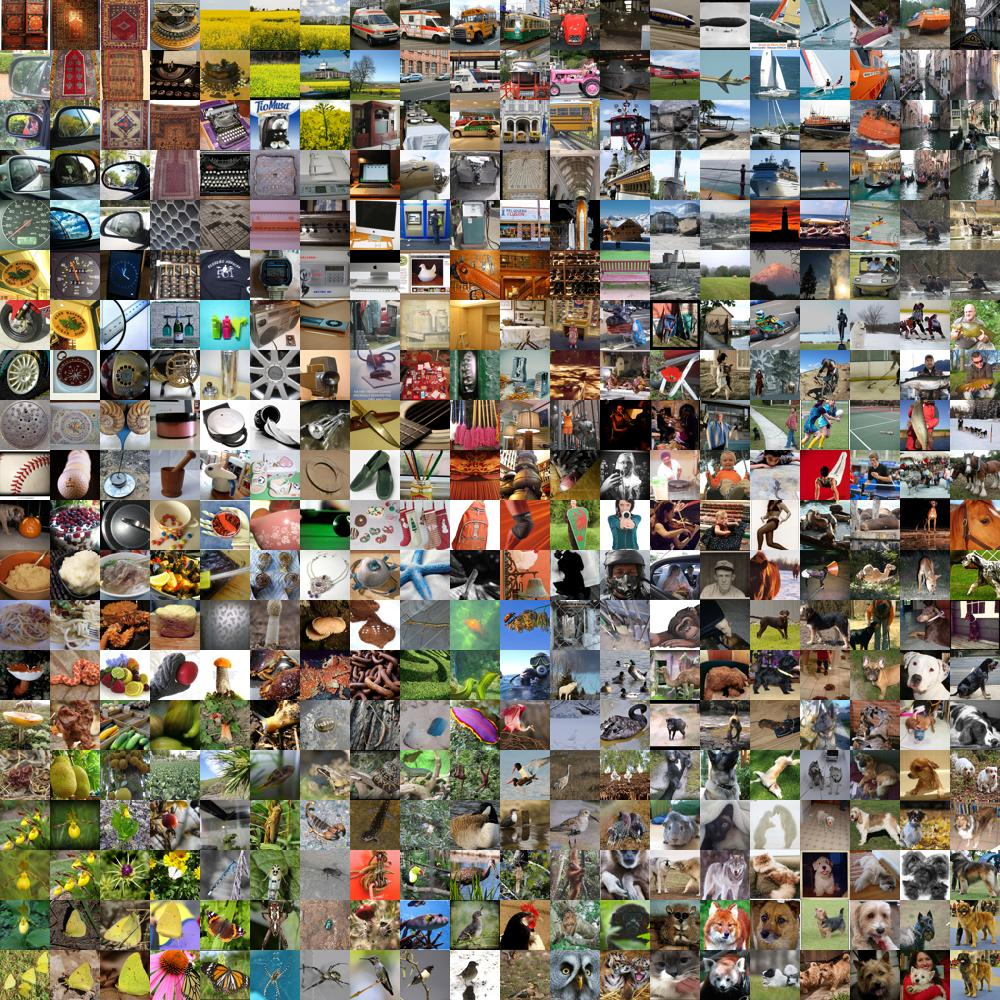
\includegraphics[scale = 0.1]{imagenet.jpg}
\end{center}
\end{column}
\begin{column}{0.4\textwidth}
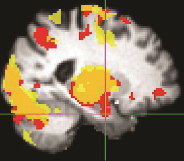
\includegraphics[scale = 0.5]{smbrain2.png}
\end{column}
\end{columns}
\vspace{0.2in}
But it would be more interesting to be able to make inferences from the data about a \emph{larger} class of stimuli...

\end{frame}

\section{Randomized classification and Average Bayes accuracy}

\begin{frame}
\sectionpage
\end{frame}

\begin{frame}
\frametitle{Randomized classification}
\begin{tabular}{c|c|c}
1. Population of stimuli $p(x)$ & 
2. Subsample $k$ stimuli &
3. Data\\
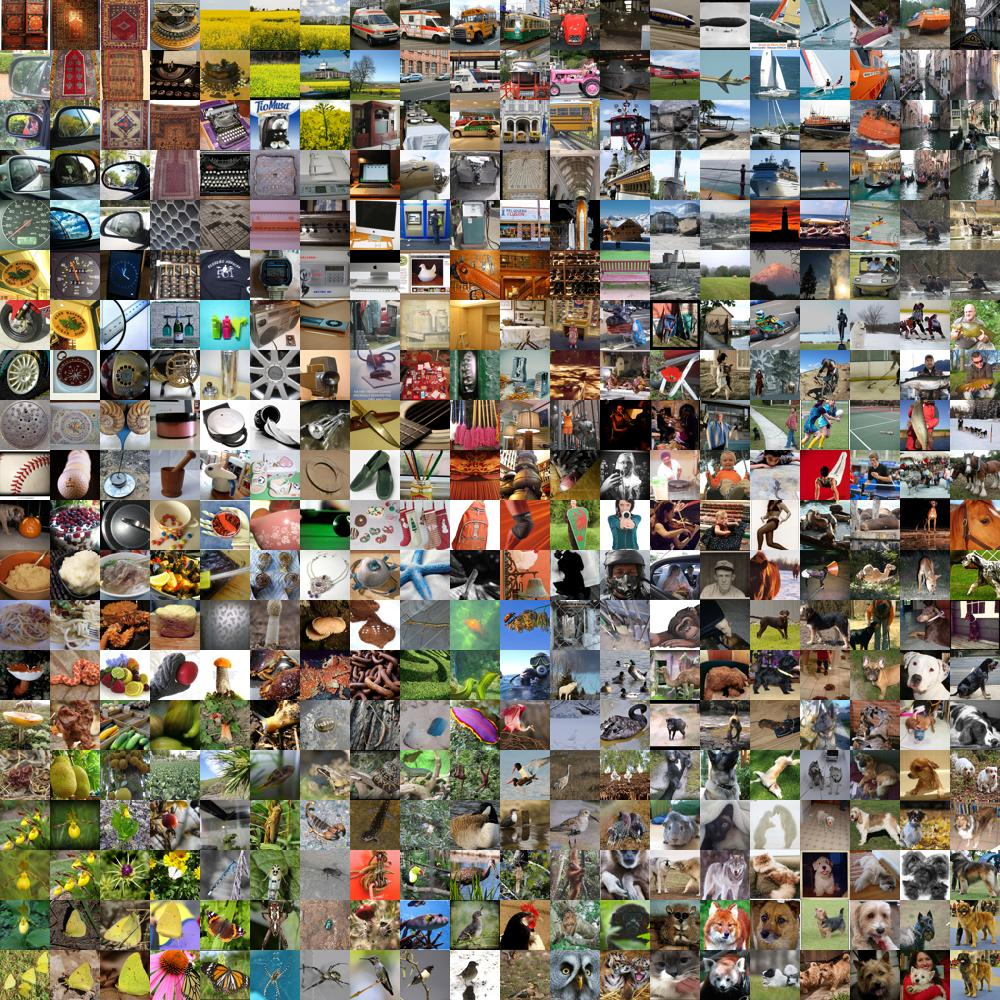
\includegraphics[scale = 0.05]{imagenet.jpg} &
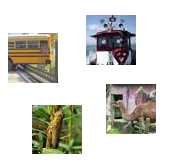
\includegraphics[scale = 0.5]{imagenet_sub.png} &
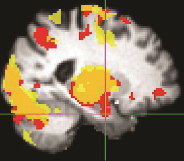
\includegraphics[scale = 0.3]{smbrain2.png}
\end{tabular}

\vspace{0.2in}
4. Train a classifier

\vspace{0.2in}
5. Estimate generalization accuracy (which is lower bound for the \emph{random} Bayes accuracy $\text{BA}_k$)
\end{frame}

\begin{frame}
\frametitle{Average Bayes accuracy}
\begin{center}
\begin{tabular}{c|c|c|c}
& Experiment 1 & Experiment 2 & Experiment 3\\\hline
&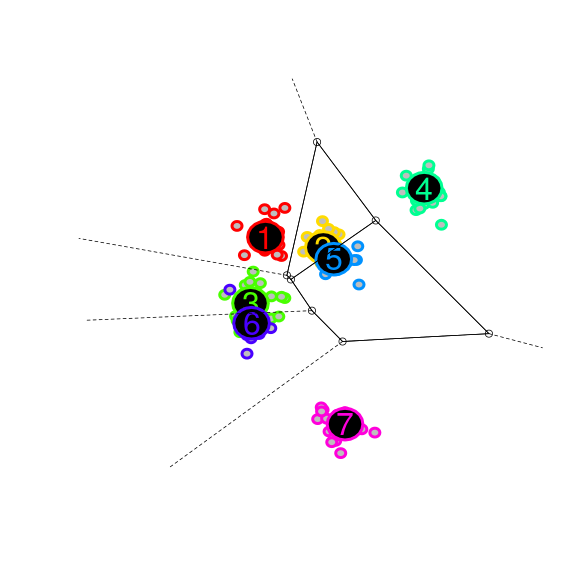
\includegraphics[scale = 0.15, clip = true, trim = 0.6in 0.2in 0.6in 0.2in]{../info_theory_paper/gaussian_figure1a.png} &
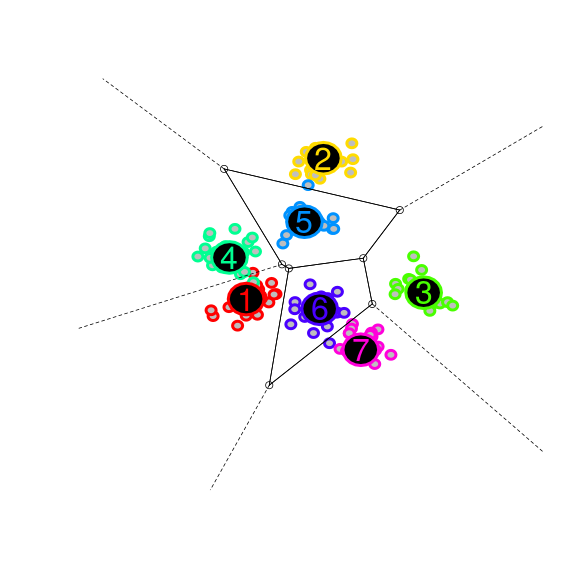
\includegraphics[scale = 0.15, clip = true, trim = 0.6in 0.2in 0.6in 0.2in]{../info_theory_paper/gaussian_figure1b.png} &
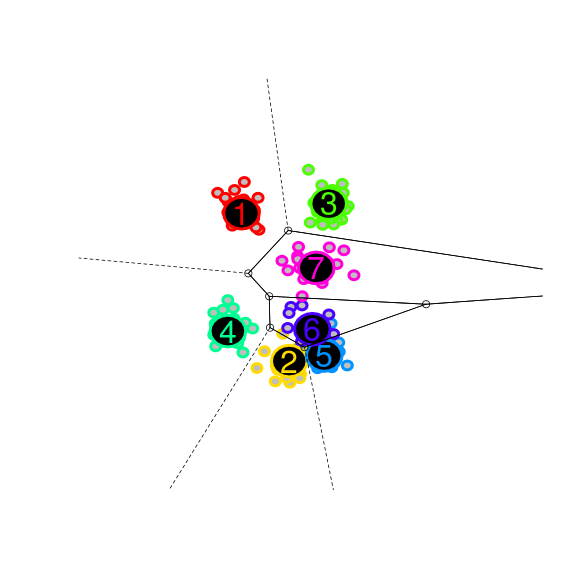
\includegraphics[scale = 0.15, clip = true, trim = 0.6in 0.2in 0.6in 0.2in]{../info_theory_paper/gaussian_figure1c.png}\\\hline
Bayes accuracy & 0.55 & 0.65 & 0.52 \\
\end{tabular}
\end{center}
\begin{itemize}
\item Bayes accuracy depends on the stimuli drawn.
\item Therefore, define $k$-class \emph{average Bayes accuracy} as the expected Bayes accuracy for $X_1,..,X_k \stackrel{iid}{\sim} p(x)$.
\[
\text{ABA}_k = \E[BA(X_1,...,X_k)]
\]
\end{itemize}
\end{frame}

\begin{frame}
\frametitle{Average Bayes accuracy}
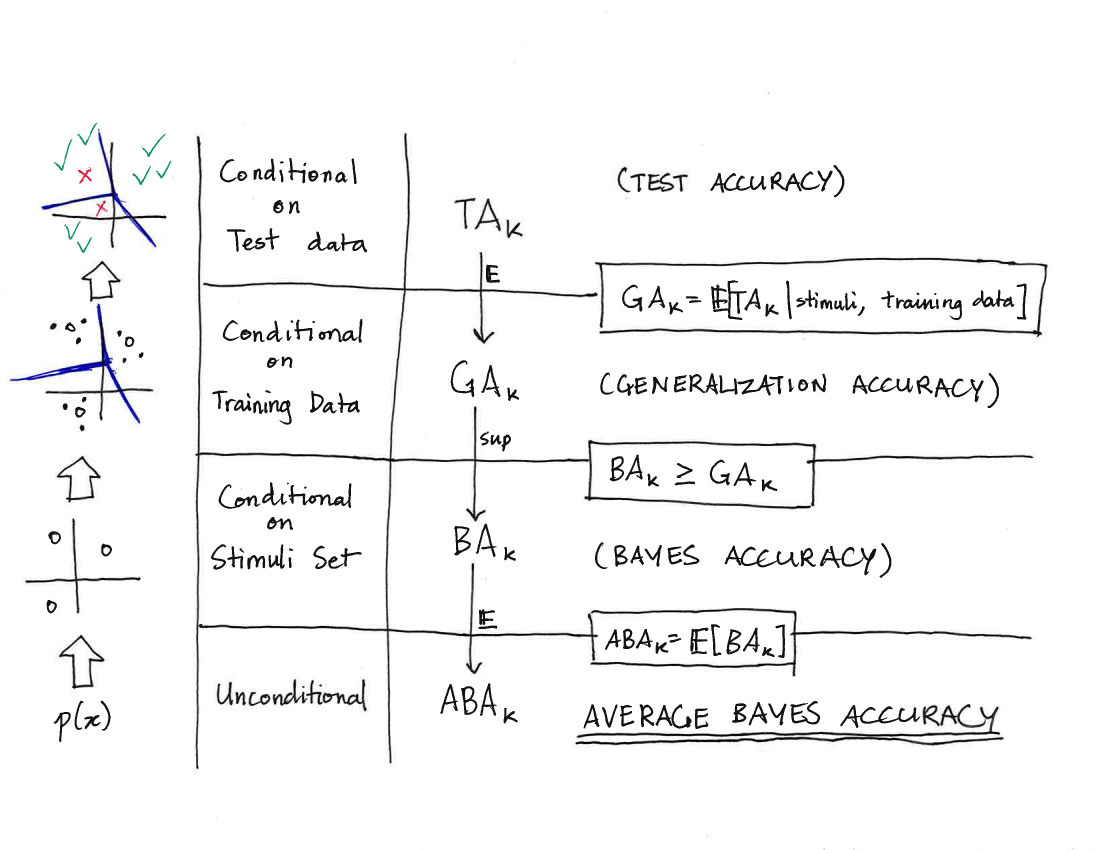
\includegraphics[scale = 0.45, clip = true, trim = 0in 1in 0.5in 1in]{ta_to_aba.png}
\end{frame}

\begin{frame}
\frametitle{Inferring average Bayes accuracy}

\begin{itemize}
\item $\text{BA}_k \stackrel{def}{=} \text{BA}(X_1,..,X_k)$ is unbiased estimate of
\[
\text{ABA}_k = \E[BA_k]
\]
by definition.
\item But what is the variance?
\[
\text{Var}[\text{BA}(X_1,...,X_k)]
\]
\item \emph{Theoretical result}. Maximal variability is of order $1/k$.
\item Therefore, it is feasbile to get a good idea of $\text{ABA}_k$ by choosing a sufficiently large sample size $k$.
\end{itemize}
\end{frame}

\begin{frame}
\frametitle{Two intuitions for variability result}
Why does variability decrease with $k$?
\begin{itemize}
\item 1. Bayes accuracy behaves like an average of $k$ i.i.d random variables. (Also gives correct $1/k$ rate.)
\item 2. Bayes accuracy behaves like a max of $k$ i.i.d. random variables.
\end{itemize}
\end{frame}

\begin{frame}
\frametitle{Intuition 1: averaging}
\begin{center}
\begin{tabular}{c|c|c|c}
& Experiment 1 & Experiment 2 & Experiment 3\\\hline
&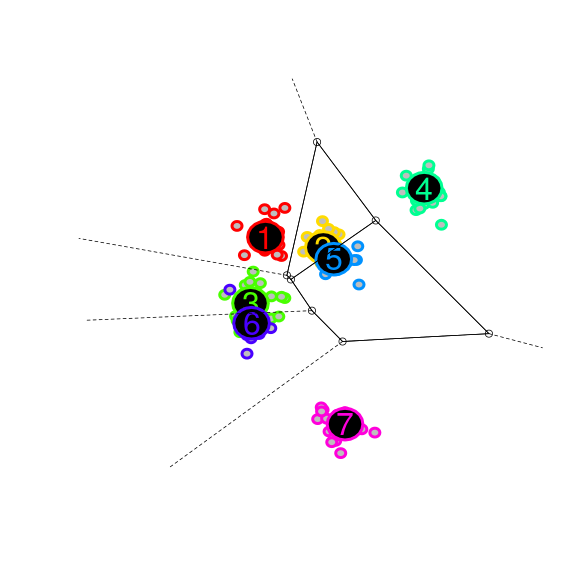
\includegraphics[scale = 0.15, clip = true, trim = 0.6in 0.2in 0.6in 0.2in]{../info_theory_paper/gaussian_figure1a.png} &
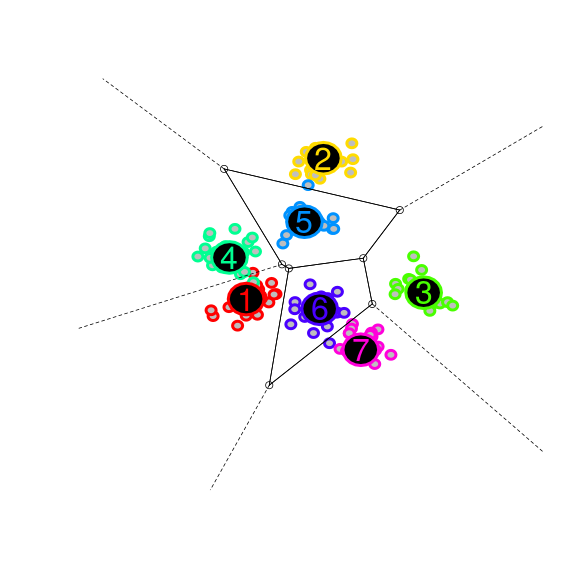
\includegraphics[scale = 0.15, clip = true, trim = 0.6in 0.2in 0.6in 0.2in]{../info_theory_paper/gaussian_figure1b.png} &
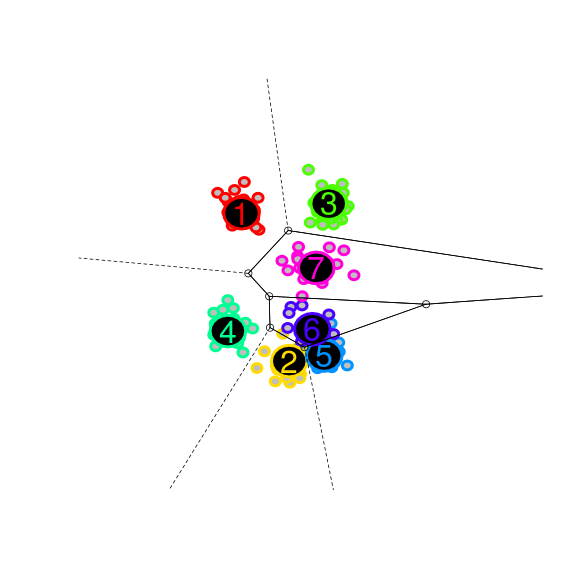
\includegraphics[scale = 0.15, clip = true, trim = 0.6in 0.2in 0.6in 0.2in]{../info_theory_paper/gaussian_figure1c.png}\\\hline
Bayes accuracy & 0.55 & 0.65 & 0.52 \\
\end{tabular}
\end{center}
Average of $k$ gaussian probability integrals... (which are asympt. uncorrelated.)
\end{frame}

\begin{frame}
\frametitle{Intuition 2: An identity}
\begin{itemize}
\item It is a well-known result from Bayesian inference that the optimal classifier $f$ is defined as
\[
f(y) = \text{argmax}_{i=1}^k p(y|x_i),
\]
since the prior class probabilities are uniform.
\item Therefore,
\begin{align*}
\text{BA}(x_1,...,x_k) &= \Pr[\text{argmax}_{i=1}^k p(y|x_i) = Z| x_1,...,x_k] 
\\&= \frac{1}{k}\int \max_{i=1}^k p(y|x_i) dy.
\end{align*}
\end{itemize}
\end{frame}

\begin{frame}
\frametitle{Intuition behind identity}
\begin{columns}
\begin{column}{0.5\textwidth}
\begin{center}
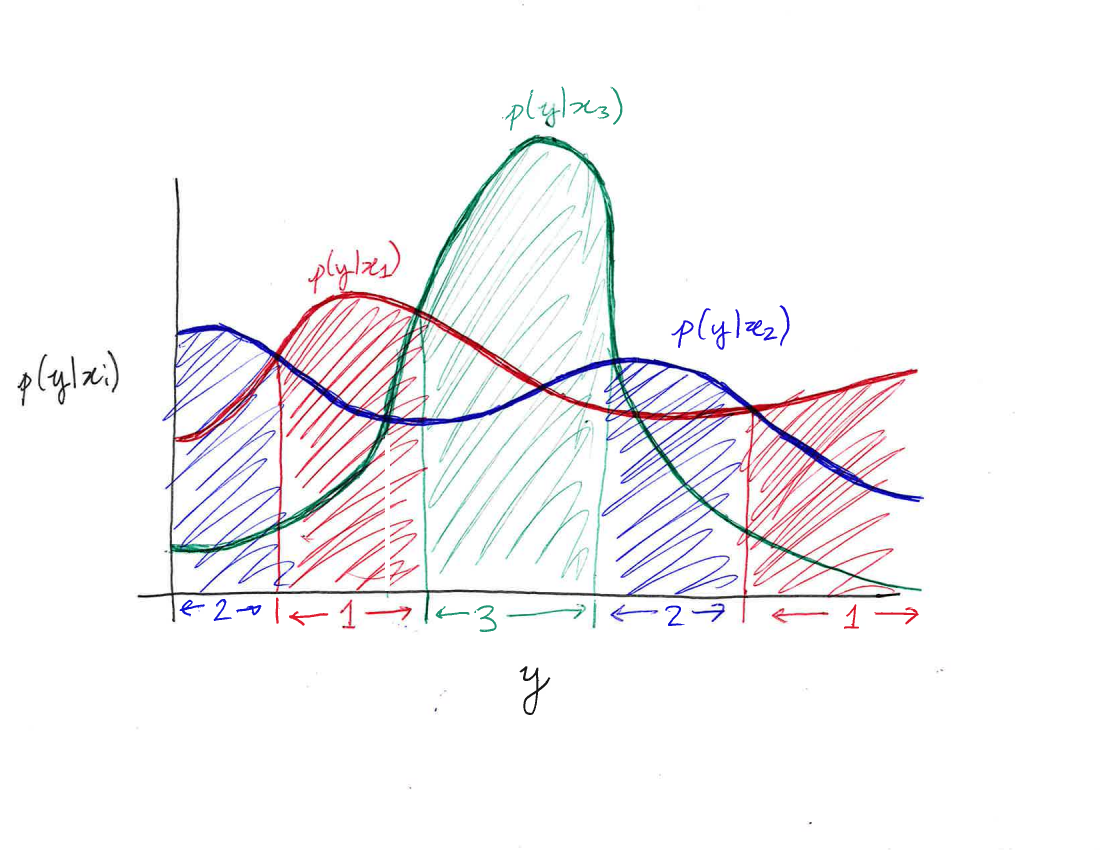
\includegraphics[scale = 0.35, clip = true, trim = 1.2in 1.3in 0in 1in]{var_ba.png}
\end{center}   
\end{column}
\begin{column}{0.5\textwidth}  %%<--- here
\begin{align*}
\text{BA}&(x_1,x_2,x_3) \\&= \sum_i \Pr[x_i]\Pr_{Y \sim p(y|x_i)}[Y \in \text{zone }i]
\\&= \sum_i \frac{1}{k} \text{Area under curve $i$ in zone $i$}
\\&\ \ \ = \frac{1}{k} \text{Area under } \max_{i=1}^k p(y|x_i)
\end{align*}
\end{column}
\end{columns}
\end{frame}

\begin{frame}
\frametitle{Variability of Bayes accuracy}

\emph{Theoretical result}. In the max formulation of $\text{BA}_k$, we
can apply Efron-Stein inequality to get
\[
\text{sd}[\text{BA}_k] \leq \frac{1}{2\sqrt{k}}
\]
\vspace{0.2in}
\emph{Empirical results}. (searching for worst-case stimuli).
\begin{tabular}{c||c|c|c|c|c|c|c}
k & 2 & 3 & 4 & 5 & 6 & 7 & 8\\\hline
$\frac{1}{2\sqrt{k}}$ & 0.353 & 0.289 & 0.250 & 0.223 & 0.204 & 0.189 & 0.177\\\hline
Worst-case sd & 0.25 & 0.194 & 0.167 & 0.150 & 0.136 & 0.126 & 0.118
\end{tabular}
\end{frame}

\begin{frame}
\frametitle{Improving the variance bound?}
\begin{itemize}
\item All of the worst-case distributions take the form
\[
\mathcal{Y} = \mathcal{X} = \{1,...,d\} \text{ for some } d
\]
\[
p(y|x) = \frac{1}{d}I\{x = y\}
\]
\item Sampling $k$ items from $d$ with replacement; $\text{BA}_k$ is the number of unique items divided by $k$.
\item According to Birthday paradox, 
\[\text{ABA}_k \approx (1-e^{-d/k})\]
and 
\[
\text{Var}(\text{BA}_k) \approx \frac{1}{d}e^{-d/k}(1-e^{-d/k})
\]
\item ``Discreteness'' of the distribution seems to maximize variance?
\item If we could prove that this is indeed the worst case, then we have a better constant for variance bound.
\end{itemize}
\end{frame}

\begin{frame}
\frametitle{Inferring average Bayes error}
For now, return to the world of finite data...
\begin{enumerate}
\item \emph{Experimental design}: draw $k$ stimuli $X_1,...,X_k$ iid from $p(x)$.  Then collect data $(X_i, Y_i^j)$.
\item \emph{Supervised learning}: train a classifier and obtain a test accuracy $\text{TA}_k$.
\item \emph{Generalization accuracy}: if $n_{test}$ is the size of the test set,
\[
\underline{\text{GA}_k} = \text{TA}_k - \frac{z_{\alpha/2}\sqrt{\text{TA}_k (1-\text{TA}_k)}}{\sqrt{n_{test}}}
\]
 is a lower confidence bound for $\text{GA}_k$
\item \emph{Bayes accuracy}:
\[
\underline{\text{BA}}_k =  \underline{\text{GA}}_k
\]
is a lower confidence bound for $\text{BA}_k$
\item \emph{Average Bayes accuracy}
\[
\underline{\text{ABA}}_k =  \underline{\text{BA}}_k - \frac{1}{2\sqrt{\alpha k}}
\]
is a lower confidence bound for $\text{ABA}_k$.
\end{enumerate}
\end{frame}

\section{Relationship between mutual information and average Bayes accuracy}

\begin{frame}
\sectionpage
\end{frame}

\begin{frame}
\frametitle{Two measures of informativity: ABA and mutual information}
Both are:
\begin{itemize}
\item measures of informativity between $X$ and $Y$
\item invariant to bijective transformations of either $X$ or $Y$
\item defined with reference to a \emph{population} of stimuli and either a single subject or population of subjects
\end{itemize}
\end{frame}

\begin{frame}
\frametitle{Comparison of ABA and mutual information}
$\text{ABA}_k$ advantages:
\begin{itemize}
\item intuitive to understand ``classification performance''.
\item easy to average over a \emph{population} of subjects.
\item closer to what you can measure: (generalization accuracy).
\end{itemize}
$\text{ABA}_k$ disadvantages:
\begin{itemize}
\item Not symmetric with respect to $X$ and $Y$.  Have to choose one as predictor and one as response.
\item Dependent on $k$, the number of classes.
\item Problem of \emph{saturation}.  If $k$ is too large,
  $\text{ABA}_k$ gets close to chance accuracy.  If $k$ is too large,
  $\text{ABA}_k$ gets close to 1.
\end{itemize}
\end{frame}

\begin{frame}
\frametitle{Comparison of ABA and mutual information}
Mutual information advantages:
\begin{itemize}
\item already has a tradition of usage in neuroscience.
\item symmetric between $X$ and $Y$: $X$ is equally informative of $Y$ as $Y$ is of $X$.
\item doesn't depend on $k$, the number of stimuli.
\item additional theoretical properties like independent additivity.
\end{itemize}
Mutual information disadvantages:
\begin{itemize}
\item not robust: $I(X; Y)$ becomes unbounded if $p(x,y)$ contains singularities.
\item does it make sense to take the average mutual information across subjects?
\end{itemize}
\end{frame}

\begin{frame}
\frametitle{Question} Given that mutual information and average Bayes
error have complementary advantages and disadvantages, can we
``convert'' one to the other?
\end{frame}

\begin{frame}
\frametitle{Related work}
\begin{itemize}
\item Classically, \emph{Fano's inequality} obtains a lower bound for
  mutual information from \emph{Bayes accuracy}.  (We do the same, but
  for \emph{average Bayes error}).
\item Treves (1997) proposes using the \emph{confusion matrix}
  obtained from classification to estimate mutual information.  This
  has been a popular approach; see Quiroga (2009).
\item Gastpar et al (2010) develop \emph{nonparametric} estimators of
  mutual information for the randomized classification setup (but does
  not involve using supervised learning.)
\end{itemize}
\end{frame}


%\begin{frame}
%\frametitle{Definitions}
%\begin{itemize}
%\item Suppose $(X, Y)$ have a joint density $p(x, y)$,
%\item The Bayes accuracy is a function of the stimuli set $x_1,...,x_k$,
%\[
%\text{BA}(x_1,...,x_k)
%\]
%\item Draw $Z \sim \{1,...,k\}$, and draw $Y \sim p(y|x_z)$.
%\item Let $f$ (the \emph{classifier}) that associates a label $\{1,...,k\}$ to each possible value of $y$:
%\[
%f: \mathcal{Y} \to \{1,...,k\}
%\]
%\item Define
%\[
%\text{BA}(x_1,...,x_k) = \sup_f \Pr[f(Y) = Z| x_1,...,x_k]
%\]
%where the probability is over the joint distribution $(Y, Z)$ defined above.
%Notice we condition on the particular stimuli set $x_1,...,x_k$.
%\end{itemize}
%\end{frame}






%\begin{frame}
%\frametitle{Efron-Stein lemma}
%\begin{itemize}
%\item We have
%\[
%\text{ABA}_k = \E[\text{BA}(X_1,...,X_k)]
%\]
%where the expectation is over the independent sampling of $X_1,...,X_k$ from $p(x)$.
%\item According to the Efron-Stein lemma,
%\[
%\text{Var}[\text{BA}(X_1,...,X_k)] \leq \sum_{i=1}^k \E[\text{Var}[\text{BA}|X_1,...,X_{i-1}, X_{i+1}, ..., X_k]].
%\]
%which is the same as
%\[
%\text{Var}[\text{BA}(X_1,...,X_k)] \leq k \E[\text{Var}[\text{BA}|X_1,...,X_{k-1}]].
%\]
%\item The term $\text{Var}[\text{BA}|X_1,...,X_{k-1}]$ is the variance of $\text{BA}(X_1,...,X_k)$
%conditional on fixing the first $k-1$ curves $p(y|x_1),...,p(y|x_{k-1})$ and allowing the final curve $p(y|X_k)$ to vary randomly.
%\end{itemize}
%\end{frame}

%\begin{frame}
%\frametitle{Efron-Stein lemma}
%\begin{itemize}
%\item 
%\[
%\text{Var}[\text{BA}(X_1,...,X_k)] \leq k \E[\text{Var}[BA|X_1,...,X_{k-1}]].
%\]
%\item Note the following trivial results
%\[
%-p(y|x_k) + \max_{i=1}^k p(y|x_i)\leq \max_{i=1}^{k-1} p(y|x_i) \leq \max_{i=1}^k p(y|x_i)
%\]
%\item This implies
%\[
%\text{BA}(X_1,...,X_k) - \frac{1}{k} \leq \frac{k-1}{k}\text{BA}(X_1,...,X_{k-1}) \leq \text{BA}(X_1,...,X_k).
%\]
%i.e. conditional on $(X_1,...,X_{k-1})$, $\text{BA}_k$ is supported on an interval of size $1/k$.
%\item Therefore,
%\[
%\text{Var}[\text{BA}|X_1,...,X_{k-1}] \leq \frac{1}{4k^2}
%\]
%since $\frac{1}{4c^2}$ is the maximal variance for any r.v. with support of length $c$.
%\end{itemize}
%\end{frame}



%\begin{frame}
%\frametitle{Intuition for variance bound}
%Write
%\[
%f(y, x_1, ..., x_k) = \text{argmax}_{i=1}^k p(y|x_i)
%\]
%so that
%\[
%\text{BA}(x_1,...,x_k) = \Pr[f(y, X_1,...,X_k) = Z| X_1 = x_1,...,X_k = x_k].
%\]
%\end{frame}

%\begin{frame}
%\frametitle{Intuition for variance bound}
%We expect the variance to be order $1/k$, because the Bayes accuracy is an average of individual class accuracies
%\[
%\text{BA}_k(X_1,...,X_k) = \frac{1}{k}\sum_{i=1}^k \Pr[f(X_1, X_2, ..., X_k, y) = Z| Z= i]
%\]
%The $i$th term,
%\[
%\Pr[f(X_1, X_2, ..., X_k, y) = Z| Z= i]
%\]
%is ``almost'' independent of the $j$th term when $k$ is large.
%Hence, since $\text{BA}_k$ is an average of $k$ ``almost-indpendent'' terms, it should have variance $\approx \frac{1}{k}.$
%\end{frame}




%\item Recalling that
%\[
%\text{BA}(X_1,...,X_k) - \frac{1}{k} \leq \frac{k-1}{k}\text{BA}(X_1,...,X_{k-1}) \leq \text{BA}(X_1,...,X_k).
%\]
%it is worth noting that distributions of this type actually
%concentrate on the two endpoints of the bound, thus in some sense
%``maximizing'' the variance.
%\item Distributions of this type actually maximize the variance
%\[\text{Var}[\text{BA}|X_1,...,X_{k-1}]\]
%given a constraint on $\E[BA|X_1,...,X_{k-1}]$,
%since 
%\[
%\text{BA}(X_1,...,X_k) = \begin{cases}
%\frac{k-1}{k}\text{BA}(X_1,..,X_{k-1}) & \text{ if }X_k \in \{X_1,..,X_{k-1}\}\\
%\frac{k-1}{k}\text{BA}(X_1,..,X_{k-1}) + \frac{1}{k} & \text{ otherwise}
%\end{cases}
%\]
%\end{itemize}
%\end{frame}

\begin{frame}
\frametitle{Natural questions}
\begin{itemize}
\item Does $\text{ABA}_k$ close to 1 imply $\text{I}$ large?
\item Does $\text{ABA}_k$ close to $1/k$ imply $\text{I}$ close to 0?
\item Does $\text{I}$ large imply $\text{ABA}_k$ close to 1?
\item Does $\text{I}$ close to $0$ imply $\text{ABA}_k$ close to $1/k$?
\end{itemize}
\end{frame}

\begin{frame}
\frametitle{Functional formulation}
Average Bayes accuracy $\text{ABA}_k[p(x, y)]$ and mutual information $\text{I}[p(x, y)]$ are both \emph{functionals} of $p(x, y)$.
\[
\text{ABA}_k[p(x, y)] = \frac{1}{k} \int p_X(x_1)\hdots p_X(x_k) \max_{i=1}^k p(y|x_i)  dx_1\hdots dx_k dy.
\]
\[
\text{I}[p(x, y)] = \int p(x, y) \log \frac{p(x, y)}{p(x)p(y)} dx dy.
\]
\end{frame}

\begin{frame}
\frametitle{Does $\text{I}$ close to $0$ imply $\text{ABA}_k$ close to $1/k$?}
Answer is yes, since $\text{I}[p(x, y)] = 0$ implies that $X$ is independent of $Y$.
And when $X \perp Y$, the best classifier does not better than random guessing.
\end{frame}

\begin{frame}
\frametitle{Does $\text{I}$ large imply $\text{ABA}_k$ close to 1?}
Answer is \textbf{no}... per the following counterexample.
\begin{columns}
\begin{column}{0.5\textwidth}
\begin{center}
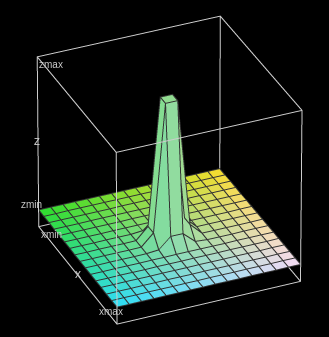
\includegraphics[scale = 0.3]{witch_hat_func.png}
\end{center}
\end{column}
\begin{column}{0.5\textwidth}
\[
X \in [0,1],\ Y \in [0,1]
\]
\[
p(x, y) \propto (1- \alpha) + \alpha \left( \frac{e^{-\frac{x^2 + y^2}{2\sigma^2}}}{2\pi\sigma^2} \right)
\]
\[
\text{I}[p(x, y)] \approx \alpha(\frac{1}{2}\log \frac{1}{\sigma^2} - 1- \log (2\pi))
\]
\end{column}
\end{columns}
Taking $\alpha \to 0$ and $\sigma^2 \leq e^{-\frac{1}{\alpha^2}}$, we get 
\[\text{I}[p(x, y)] \to \infty,\ \ \text{ABA}_k[p(x, y)] \to \frac{1}{k}.\]
This also answers ``\emph{Does $\text{ABA}_k$ close to $1/k$ imply $\text{I}$ close to 0?''} (Also no.)
\end{frame}

\begin{frame}
\frametitle{Natural questions}

\begin{itemize}
\item Does $\text{ABA}_k$ close to $1/k$ imply $\text{I}$ close to 0? \textbf{No}. (counterexample)
\item Does $\text{I}$ large imply $\text{ABA}_k$ close to 1?  \textbf{No}. (counterexample)
\item Does $\text{I}$ close to $0$ imply $\text{ABA}_k$ close to $1/k$? \textbf{Yes}.
\end{itemize}

The only remaining question is:
\vspace{0.2in}

Does $\text{ABA}_k$ close to 1 imply $\text{I}$ large?
\vspace{0.2in}

The answer is yes and provides an ``extension'' of Fano's inequality.  Unlike in Fano's inequality,
\[
\text{ABA}_k \to 1
\]
implies
\[
\text{I}[p(x, y)] \to \infty.
\]
\end{frame}

\begin{frame}
\frametitle{Problem formulation} Take $\iota > 0$, and fix $k \in
\{2,3,...\}$.  Let $p(x, y)$ be a joint density (where $(X, Y)$
could be random vectors of any dimensionality.)  Supposing
\[
\text{I}[p(x, y)] \leq \iota,
\]
then can we find an upper bound on $\text{ABA}_k[p(x, y)]$?

In other words, can we compute the value of
\[
C_k(\iota) = \sup_{p(x, y): \text{I}[p(x, y)] < \iota} \text{ABA}_k[p(x, y)]?
\]
\end{frame}

\begin{frame}
\frametitle{Preview}

Yes we can, and this is what the resulting function $C_k(\iota)$ looks like:
\begin{center}
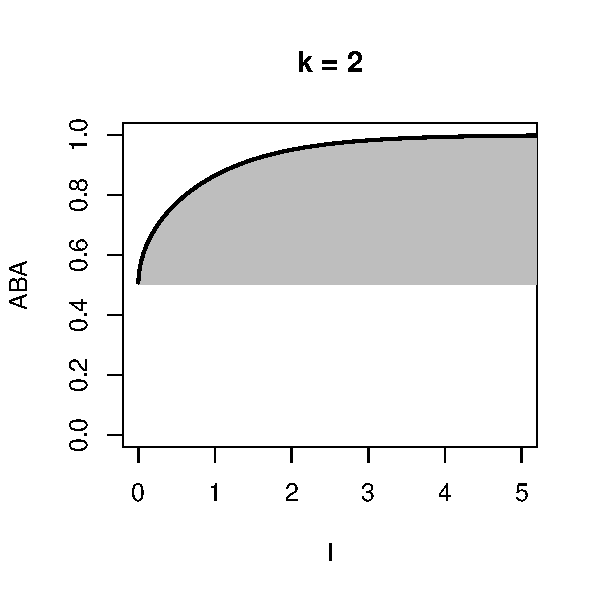
\includegraphics[scale = 0.34]{ck_2.pdf}
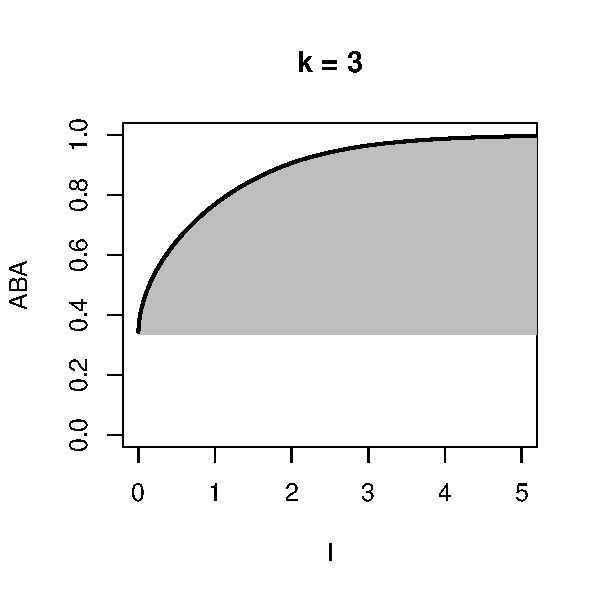
\includegraphics[scale = 0.34]{ck_3.pdf}
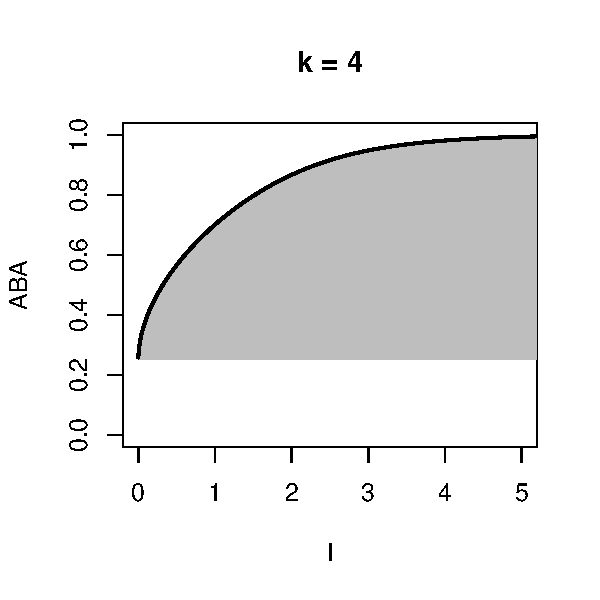
\includegraphics[scale = 0.34]{ck_4.pdf}
\end{center}
As information increases, the maximal average Bayes accuracy goes to 1.

%We find these curves using \emph{variational calculus}.

\end{frame}

\begin{frame}
\frametitle{Reduced Problem}
Rather than show the whole proof, we consider a simplified problem to illustrate the methods.
\begin{center}
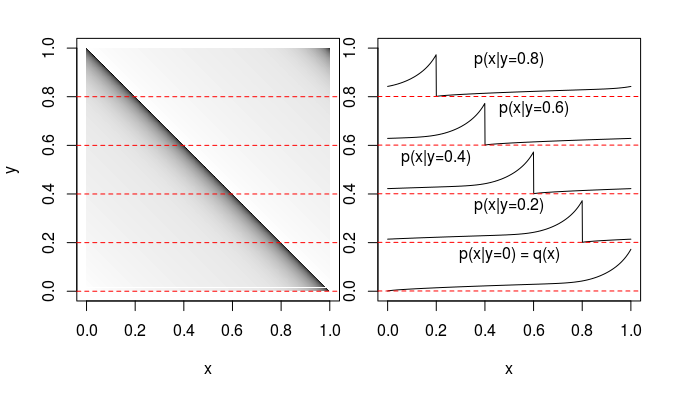
\includegraphics[scale = 0.5]{../diagram/qxplot.png}
\end{center}

Actually, the simplified problem is equivalent to the full problem and we get the same answer (but this is non-trivial).
\end{frame}

\begin{frame}
\frametitle{Reduced Problem}

\begin{center}
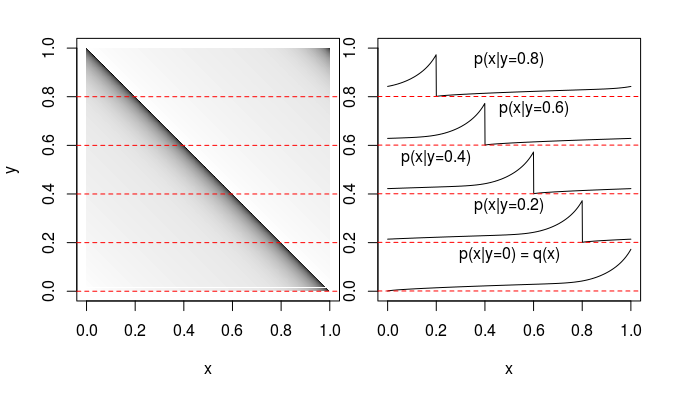
\includegraphics[scale = 0.4]{../diagram/qxplot.png}
\end{center}

\begin{itemize}
\item $p(x, y)$ on unit square with uniform marginals.
\item The conditional distributions $p(x|y)$ are just ``shifted'' copies of a common density, $q(x)$, on $[0,1]$
\[
p(x|y) = q(x - y + I\{x < y\})
\]
\item Furthermore, $q(x)$ is increasing in $x$.
\end{itemize}


\end{frame}

\begin{frame}
\frametitle{Simplified formulae}

The information and average Bayes error can be written in terms of $q(x)$.

\[
\text{I}[p(x, y)] = \int_0^1 q(x) \log q(x) dx
\]
\[
\text{ABA}_k[p(x, y)] = \int_{[0, 1]^k} \max_{i=1}^k q(x_i) dx_1 \cdots dx_k
\]

\end{frame}

\begin{frame}
\frametitle{Simplified formulae}

Overload the notation and ``redefine'' information and average Bayes error as functionals of $q(x)$.

\[
\text{I}[q(x)] \stackrel{def}{=} \int_0^1 q(x) \log q(x) dx
\]
\[
\text{ABA}_k[q(x)] \stackrel{def}{=} \frac{1}{k}\int_{[0, 1]^k} \max_{i=1}^k q(x_i) dx_1 \cdots dx_k
\]

\end{frame}

\begin{frame}
\frametitle{Simplified formulae}

We can simplify the expression for $\text{ABA}_k$ even more.

Observe that since $q(x)$ is increasing,
\[
\max_{i=1}^k q(x_i) = q\left(\max_{i=1}^k x_i\right)
\]

Therefore,
\begin{align*}
\text{ABA}_k[q(x)] &= k^{-1}\int_{[0, 1]^k} \max_{i=1}^k q(x_i) dx_1 \cdots dx_k
\\&= k^{-1}\int_{[0, 1]^k} q\left(\max_{i=1}^k x_i\right) dx_1 \cdots dx_k
\\&= k^{-1}\E\left[q\left(\max_{i=1}^k X_i\right)\right] = k^{-1}\E[q(M)]
\end{align*}
where $X_1,\hdots, X_k \stackrel{iid}{\sim} \text{Unif}[0,1]$ and $M = \text{max}_{i=1}^k X_i$.

\end{frame}

\begin{frame}
\frametitle{Simplified formulae}

Recall that the max of $k$ iid uniforms has density
\[
f(m) = km^{k-1}.
\]
Therefore,
\begin{align*}
\text{ABA}_k[q(x)] =  k^{-1}\E[q(M)] = \int_0^1 q(t) t^{k-1} dt.
\end{align*}

\end{frame}


\begin{frame}
\frametitle{Optimization problem}
We now pose the question: how do we find $q(x)$ which maximizes $\text{ABA}_k[q(x)]$ subject to $\text{I}[q(x)] \leq \iota$?

\begin{itemize}
\item \emph{Domain of the optimization}: Recall that $q(x)$ satisfies $q(x) \geq 0$, $\int_0^1 q(x) dx = 1$, and is increasing in $x$.
Let $\mathcal{Q}$ denote the space of functions on $[0,1] \to [0,\infty)$ which are increasing in $x$.
\item \emph{Constraints}: We have two remaining constraints, $\text{I}[q(x)] \leq \iota$ and $\int_0^1 q(x) dx = 1$.
\end{itemize}

Hence the problem is
\[
\text{maximize}_{q(x) \in \mathcal{Q}}\text{ ABA}_k[q(x)]\text{ subject to }\int_0^1 q(x) dx = 1\text{ and }\text{I}[q(x)] \leq \iota.
\]
\end{frame}

\begin{frame}
\frametitle{Optimization problem}
\[
\text{maximize}_{q(x) \in \mathcal{Q}}\text{ ABA}_k[q(x)]\text{ subject to }\int_0^1 q(x) dx = 1\text{ and }\text{I}[q(x)] \leq \iota.
\]
\begin{itemize}
\item Does a solution exist? \emph{Yes}, because the space of measures
  with density $q(x)$ satisfying $\text{I}[q(x)] \leq \iota$ is tight,
  and both the constraints and objective are continuous wrt to the
  topology of weak convergence.
\item Given a solution $q^*(x)$ exists, there exist Lagrange multipliers $\lambda \in \mathbb{R}$ and $\nu > 0$ such that $q^*$ minimizes
\begin{align*}
\mathcal{L}[q(x)] &= -\text{ABA}_k[q(x)] + \lambda \int_0^1 q(x) dx + \nu \text{I}[q(x)]
\\&= \int_0^1 (-t^{k-1} + \lambda + \nu \log q(x)) q(x) dx.
\end{align*}
\end{itemize}

\end{frame}

\begin{frame}
\frametitle{Functional derivatives}
\begin{itemize}
\item Functional derivatives are essential to variational calculus.
\item Let $\mathcal{F}$ be a \emph{Hilbert space} of functions with domain $\mathcal{X}$ and range $\mathbb{R}$.
\item Suppose $F$ is a functional which maps functions $f$ to the real line.
Then the functional derivative $\nabla F[f]$ at $f$ is a function in the space $\mathcal{F}$ such that
\[
\lim_{\epsilon \to 0}\frac{F(f + \epsilon \xi) - F(f)}{\epsilon} = \int_{\mathcal{X}} \nabla F[f](x) \xi(x) dx.
\]
for all $\xi \in \mathcal{F}$.
\end{itemize}
\end{frame}

\begin{frame}
\frametitle{Functional derivatives}
\begin{itemize}
\item Taylor explansions are a useful trick for computing functional derivatives
\item We can compute the functional derivative of $\mathcal{L}[q(x)]$ by writing
\begin{align*}
\mathcal{L}[q(x) + \epsilon \xi(x)] &
\\= \int_0^1 (-t^{k-1} &+ \lambda + \nu \log (q(x) + \epsilon \xi(x))) (q(x) + \epsilon \xi(x)) dx.
\\\approx  \int (q(x) + &\epsilon \xi(x)) (-t^{k-1} + \lambda + \nu \{\log q(x) + \frac{\epsilon \xi(x)}{q(x)}\}) dx
\\\approx  \mathcal{L}[q(x)] +& \int_0^1 (-t^{k-1} + \lambda + \nu (1 + \log q(x)) \epsilon\xi(x) dx.
\end{align*}
\item Hence
\[
\nabla \mathcal{L}[q](x) = -t^{k-1} + \lambda + \nu (1 + \log q(x))
\]
\end{itemize}
\end{frame}


\begin{frame}
\frametitle{Variational magic!}
Suppose we set the functional derivative to 0,
\[
0 = \nabla \mathcal{L}[q](t) = -t^{k-1} + \lambda + \nu + \nu \log q(t).
\]
Then we conclude that the optimal $q^*(t)$ takes the form
\[
q^*(t) = \alpha e^{\beta t^{k-1}}
\]
for some $\alpha > 0$, $\beta > 0$.

From the constraint $\int q(t)dt = 1$, we get
\[
q_\beta(t) = \frac{e^{\beta t^{k-1}}}{\int e^{\beta t^{k-1}} dt}.
\]
\end{frame}

\begin{frame}
\frametitle{Technical sidenote}
\textbf{For the optimal $q(t)$, how do we know $\nabla \mathcal{L}[q](t) = 0$?}

\begin{itemize}
\item Since $\mathcal{Q}$ has a monotonicity constraint, we cannot simply take for granted that
\[
\nabla \mathcal{L}[q^*](t) = 0
\]
\item However, we can show that assuming 
\[
\nabla \mathcal{L}[q^*](t) \neq 0
\]
on a set of positive measure results in a contradiction.
\item The contradiction is achieved by constructing a suitable
  perturbation $\xi$ which is ``localized'' around a region where
  $\mathcal{L}[q^*](t)\neq 0$, such that $q^* + \epsilon \xi \in
  \mathcal{Q}$ and also so that $\int \xi(t) \nabla
  \mathcal{L}[q^*](t) dt < 0$.  This implies that for $\epsilon$
  sufficiently small, $\mathcal{L}[q^* + \epsilon \xi] <
  \mathcal{L}[q^*]$--a contradiction, since we assumed that $q^*$ was
  optimal.
\end{itemize}
\end{frame}

\begin{frame}
\frametitle{Result}
\textbf{Theorem}.
For any $\iota > 0$, there exists $\beta_\iota \geq 0$ such that defining
\[
q_\beta(t) = \frac{\exp[\beta t^{k-1}]}{\int_0^1 \exp[\beta t^{k-1}]},
\]
we have
\[
\int_0^1 q_{\beta_\iota}(t) \log q_{\beta_\iota}(t) dt = \iota.
\]
Then,
\[
C_k(\iota) = \int_0^1 q_{\beta_\iota}(t) t^{k-1} dt.
\]
\end{frame}

\begin{frame}
\frametitle{Conclusion: Inferring mutual information from randomized classification}
\begin{columns}
\begin{column}{0.5\textwidth}
\begin{itemize}
\item Step 1: Apply machine learning to obtain \emph{test accuracy} $\text{TA}_k$.
\item Step 2: Obtain lower confidence bound $\underline{\text{ABA}_k}$.
\item Step 3: Obtain a lower confidence bound on $I(X; Y)$ from $\underline{\text{ABA}_k}$.
\end{itemize}
\end{column}
\begin{column}{0.5\textwidth}
\begin{center}
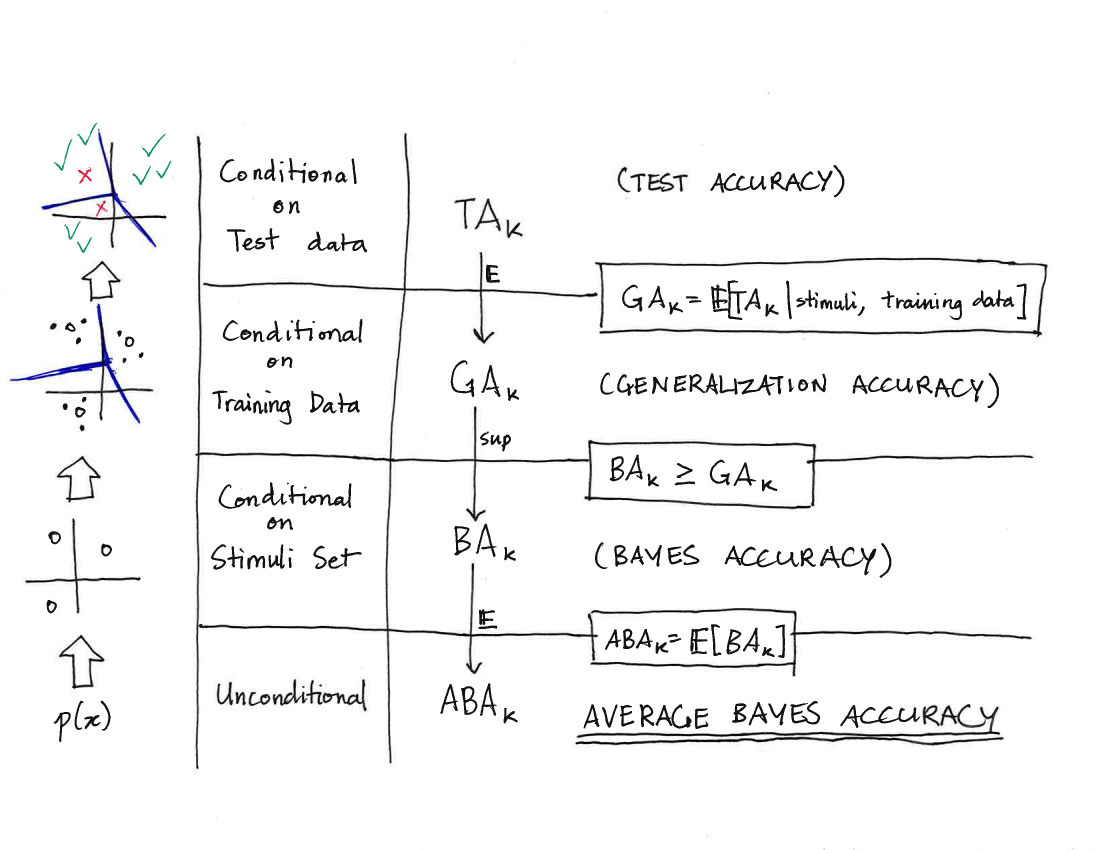
\includegraphics[scale = 0.3, clip = true, trim = 0in 1in 5.5in 1in]{ta_to_aba.png}
\end{center}   
\end{column}
\end{columns}
\end{frame}

\begin{frame}
\frametitle{The end}
\begin{center}
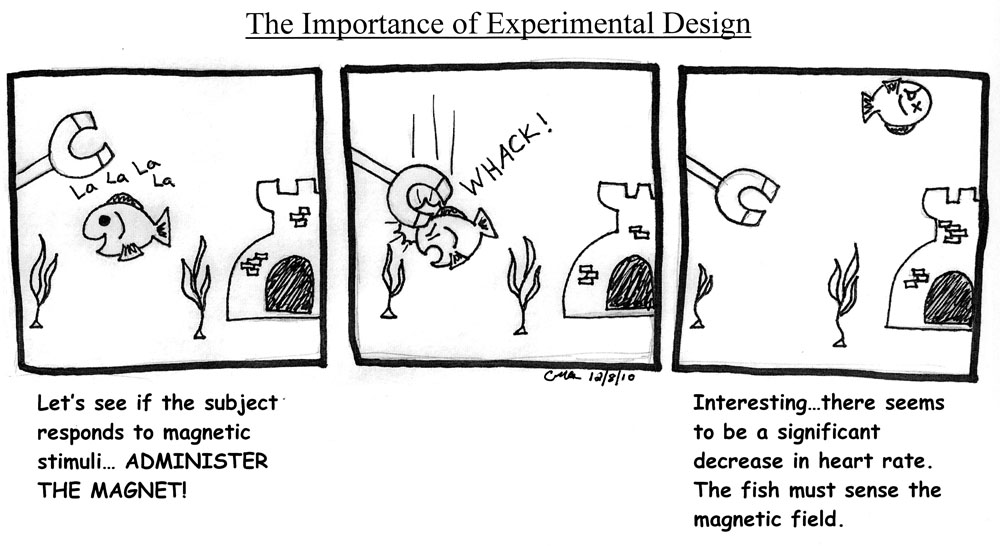
\includegraphics[scale = 1]{c_ambrosino.jpg}


{\tiny(credit C. Ambrosino)}
\end{center}
\end{frame}

\begin{frame}
\frametitle{Fun fact: ``variational'' proof of Fano's inequality}
$X \sim \text{Unif}\{1,...,k\}$, $Y \sim \text{Unif}[0,1]$.
\[
\text{I}(X; Y) = \frac{1}{k}\sum_x \int p(y|x) \log p(y|x) dy,
\]
\[
\text{BA} = \frac{1}{k} \int \max_x p(y|x) dy.
\]
reduces to
\[
\text{maximize}_{q_i \geq 0}\ \max_{i=1}^k q_i\]
\[ \text{ s.t. }\sum_{i=1}^k q_i =  1\text{ and }\log(k) + \sum_{i=1}^k q_i \log q_i\leq \iota.
\]
\end{frame}

\begin{frame}
\frametitle{Fun fact: ``variational'' proof of Fano's inequality}
Optimum takes the form
\[
q_1 = \beta,\ q_2 =\cdots=q_k = (1-\beta)/(k-1).
\]
where $\text{BA} = \beta$.
Hence,
\begin{align*}
\text{I}(X; Y) &\leq \iota = \log(k) + \beta \log(\beta) + (1-\beta)\log((1-\beta)/(k-1))
\\&= \log(k)-H(\text{BA}) - (1-\text{BA})\log(k-1),
\end{align*}
which is Fano's inequality.
\end{frame}

\end{document}
